\section{Experiments and Evaluation}
TODO: dataset
\subsection{Dimension reduction}
Our first set of experiments featured the basic dimension reduction method,
without the modifications for compression. We were looking to verify that the
required reconstruction information was present within the lower dimensional
representation created by the feature extractor. (TODO include bitrate) The
qualitative results can be seen in Figure 1. \\

We also utilized our latent loss scheme by pre-training on image reconstruction
before training on the latent loss. The results can be seen in Figure 2.
\begin{figure}[H]
    \centering
    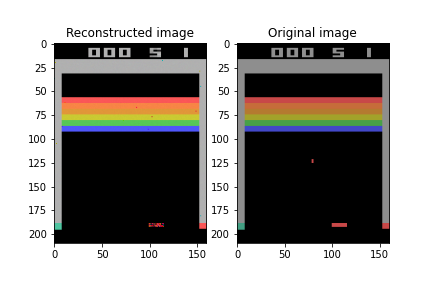
\includegraphics[width=0.6\textwidth]{images/orig_reconstructed0.0.png}
    \caption{Baseline method (no compression) with decoder trained on MSE for 10,000 iterations}
    \label{fig:baseline_MSE}
\end{figure}
\begin{figure}[H]
    \centering
    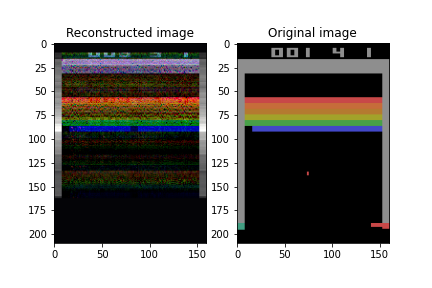
\includegraphics[width=0.6\textwidth]{images/orig_reconstructed_rl3.0.png}
    \caption{Baseline method (no compression) with decoder trained on MSE for 10,000 iterations, then latent MSE for 10,000 iterations}
    \label{fig:baseline_MSE_latent}
\end{figure}

\subsection{Compression}
Now we added the compression loss to the training of the RL agent
\ref{eq:RL_Training_Loss} and trained the agent with this loss function. We
modified the $\alpha$ value, the idea beeing that larger alpha values give a
larger penalty and therefore higher compression. Ultimatly however, the
performance of the Encoder together with the Decoder is important, a too high
compression would destroy too much information. %TODO: That is true but alpha in our case wasnt stabely changing compression performance

An alpha of $1e-8$ TODO: verify seemed to work best for the Decoder, therefore
we chose this value for an extended run over ... TODO: add epochs. Tested on an
independently created test dataset, this resulted in an entropy of 1.7 bits per
latent dimension, if the latent values get rounded to 3 digits. The actual
bitrate given as the cross-entropy \ref{eq:BitRate} is higher however, since
we need to choose a fixed distribution for encoding and transmission of the
latents. As for training we chose a normal distribution with mean 0 and learned
variance, we also use this for testing. The expected variance per dimension was
estimated by the mean per dimnesion over the whole test dataset. However the
cross entropy over the test dataset was infinity. A visual investigation of the
latent values showed that while the entropy of the latent values was low, some
of the values deviated of 0 significantly, (in the order of 100), which led to a
probability of nearly 0 and a logprob of -infinity.

After training the RL Agent, the decoder was trained for ... TODO: add epochs.
This resulted in an MSE Loss of 1895 or 2322 ?? TODO. As discussed in
\ref{sec:Introduction}, MSE Loss is not a good metric for performance, since it
gives each pixel the same value. Therefore we investigated some images. An
example can be seen in figure \ref{fig:final_agent}. The image shows that during
compression some of the data got lost, since the image is distorted.
\begin{figure}[H]
    \centering
    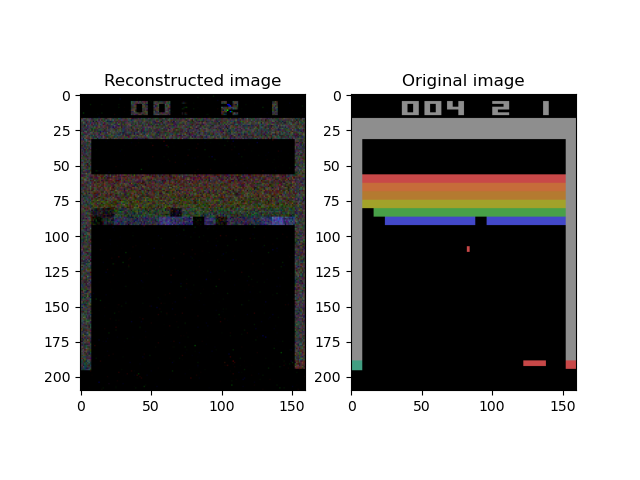
\includegraphics[width=0.6\textwidth]{images/orig_reconstructed_final_agent.png}
    \caption{Baseline method (no compression) with decoder trained on MSE for 10,000 iterations}
    \label{fig:final_agent}
\end{figure}

\subsection{Adaptive Alpha}
When we implemented our custom loss function with static $\alpha$, several
rudimentary tests were done to verify that the model behaved as expected. One
such test involved varying $\alpha$: we expected that a lower value would
prioritize task performance, while a higher value would prefer a lower bitrate.
However, we found this was not the case: there seemed to be just as much
variation between independent tests of the same $\alpha$ as changing $\alpha$
(add results in appendix?). Given our hypothesis for where the problem lay (see
Methods), we developed the adaptive $\alpha$ scheme. However, initial results
showed no improvement and we were forced to move this to Future Work.

\subsection{Pretrained agents}
Another idea was that maybe adding the compression loss to the RL agent from the
beginning on was a too large constrain for the agent to learn anything.
Therefore, we tried to fix this by first pretraining the agent, and then adding
the compression loss to the agent. On the one hand, the compression loss reduced
the entropy but on the other hand, the decoder couldn't learn anymore, so this
procedure showed no improvements.




% TODO:

% structure eval:
% - show compression performance, maybe the curve
% - show that while entropy is low, cross entropy still high for final agent (overfit?)
% - show some images during training, agent can learn paddle position, not only memorize images
% - show that it breaks down for evaluation set

% other experiments:
% - github code: scaled noise together with variance
% - write up pretrained agent that was trained on, but info just destroyed

